
\begin{center}
\begin{tabular}{c}
\covtitle{ERC Starting Grant 2021} \\[.3em]
\covtitle{Research Proposal [Part B1]} \\[1.5em]
\lntitle{
Satisfiability Modulo Theories and Automated Theorem Proving:}\\[.3em]
\lntitle{Quest for Unity} \\[1em]
\lntitle{UNIFAR}
\end{tabular}
\end{center}

\bigskip
\noindent
\begin{tabular}{ll}
Principal investigator (PI) & Shachar Itzhaky \\[.5em]
Host institution & Technion, Israel Institute of Technology \\[.5em]
Proposal duration: & 60 months
\end{tabular}

\bigskip\noindent
\fbox{\parbox{0.95\textwidth}{
\quad Automated reasoning using mathematical logic constitutes a large chunk of today's software analysis and verification.
It is front and center in any automatic verifier, as well as a core component in automatic test generation and synthesis tools.
At present, there exist two predominant approaches to automated reasoning:
\emph{automated theorem proving} (ATP) and
\emph{satisfiability modulo theory} (SMT).
They have somewhat converged toward a common goal, namely, proving the validity of a logical proposition.
However, over the last twenty years, they have significantly diverged in the techniques used to attain this goal,
to the point where sharing and porting ideas between them is almost never done anymore,
due to a gap in mathematical terminology and formal calculi being used.
Since each such technique has its own strengths and weaknesses, some problems are solved easily using one tool, but cannot be solved at all by the other.
This difficulty raises the need to form a \textbf{unifying framework for automated reasoning},
that will be able to describe both ATPs and SMT solvers on top of a common mathematical foundation.
This proposal embodies a quest for the \textbf{missing link} connecting the ATP and SMT camps,
\textbf{bridging the gap} between them.
This is imperative for cross-fertilization of ideas,
and is a vital ingredient in pushing automated reasoning technology forward.

\quad This research proposes to build on recent developments in computational logic, such as advances in Type Theory, cyclic proofs, and theory exploration, to yield theories and algorithms that will lead to a new generation of automated reasoning tools.
By concentrating effort on proof scenarios that arise from dealing with programming-language semantics and software specifications,
we aspire to \textbf{break the barrier that currently blocks software verification} from scaling up and becoming suitable for real-world applications.
}}

\vspace{3cm}
\begin{center}
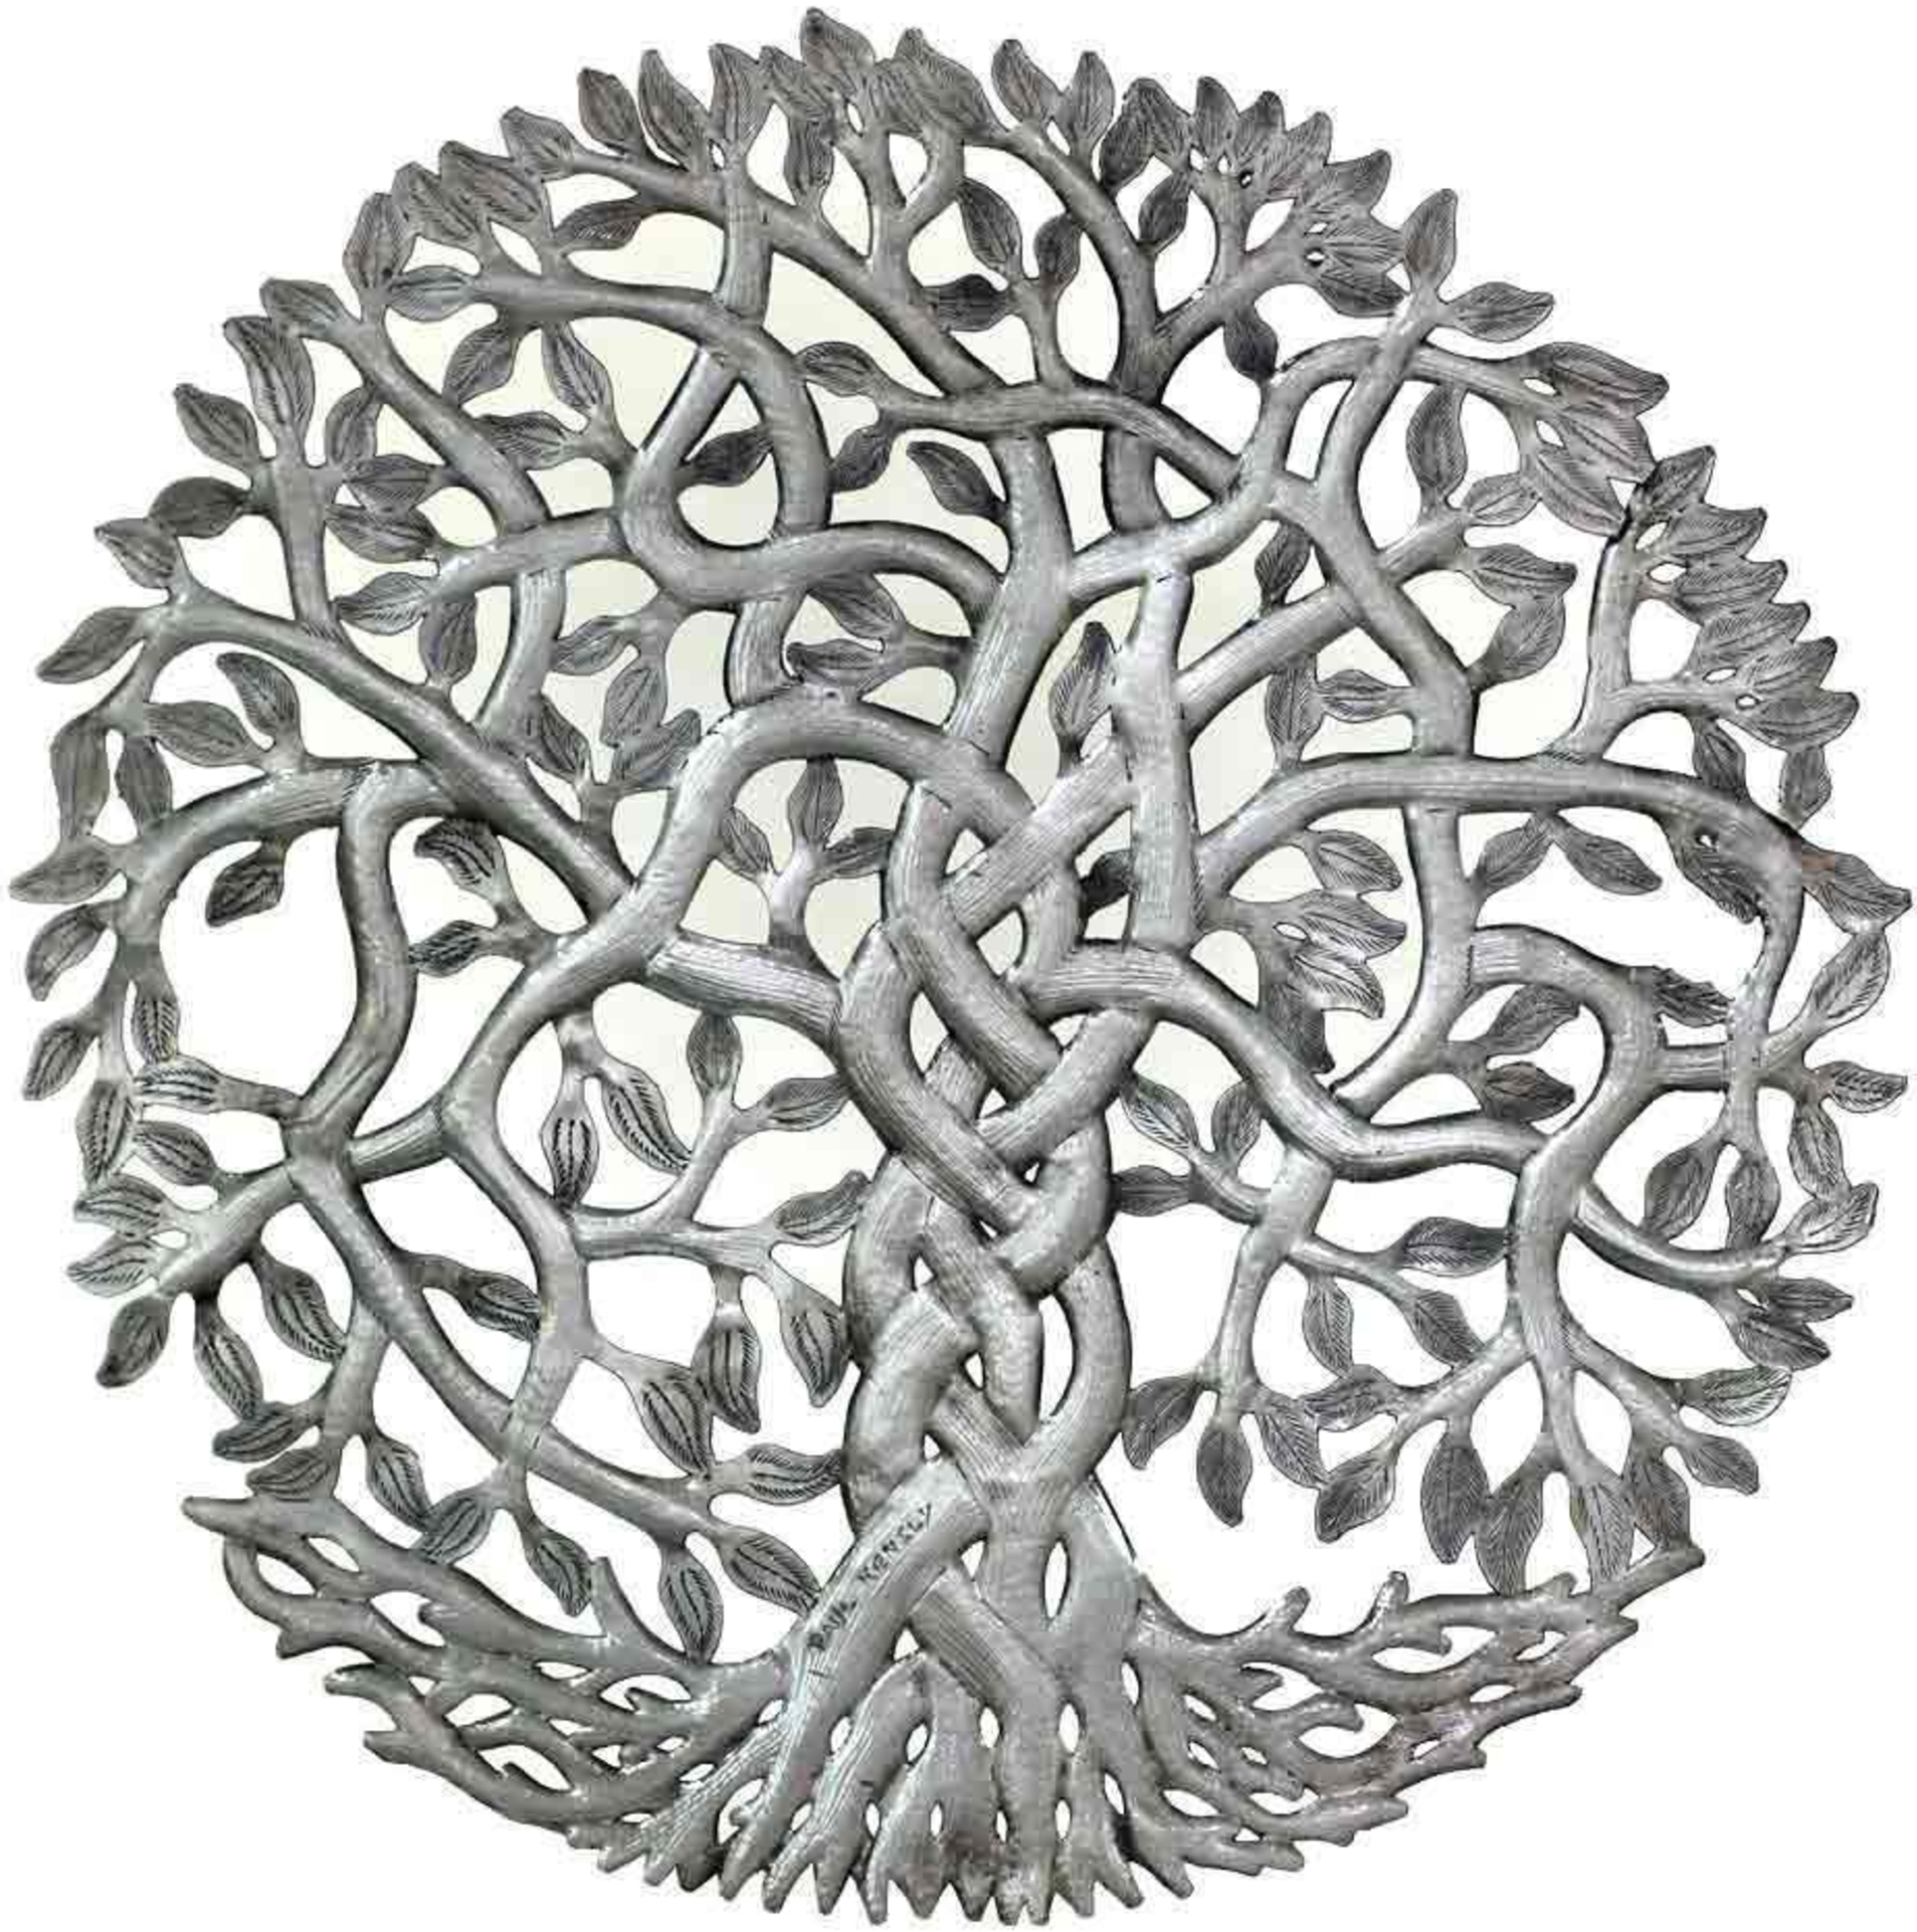
\includegraphics[width=5cm]{img/entangled-tree-of-life.pdf}
\end{center}


\clearpage